\documentclass[conference]{IEEEtran}
\IEEEoverridecommandlockouts
% The preceding line is only needed to identify funding in the first footnote. If that is unneeded, please comment it out.
\usepackage{cite}
\usepackage{amsmath,amssymb,amsfonts}
\usepackage{algorithmic}
\usepackage{graphicx}
\usepackage{textcomp}
\usepackage{xcolor}
\usepackage[backend=bibtex]{biblatex}
\addbibresource{References.bib}

\usepackage{listings}
\usepackage{xcolor}
\usepackage{caption}
\usepackage{booktabs}
\lstset{
  basicstyle=\ttfamily\footnotesize,
  backgroundcolor=\color{gray!10},
  frame=single,
  breaklines=true
}

\usepackage{tabularx}
\usepackage{adjustbox}


\def\BibTeX{{\rm B\kern-.05em{\sc i\kern-.025em b}\kern-.08em
    T\kern-.1667em\lower.7ex\hbox{E}\kern-.125emX}}
\begin{document}

\title{ Dynamic Sporadic Server\\

}

\author{\IEEEauthorblockN{ Moiz Zaheer Malik}
\IEEEauthorblockA{\textit{ B.Eng. Electronic Engineering} \\
\textit{Hochschule Hamm-Lippstadt}\\
Lippstadt, Germany \\
moiz-zaheer.malik@stud.hshl.de}

}

\maketitle

\begin{abstract}
In real-time systems, where tasks have different levels of critical importance, it is essential to serve aperiodic (irregular, event-driven) tasks while ensuring that the deadlines of high-priority periodic tasks are not violated. The Dynamic Sporadic Server (DSS) is a scheduling method designed for Earliest Deadline First (EDF) systems that addresses this problem. 

DSS is defined by a period  $T_s$ and a budget $C_s$, but unlike traditional sporadic servers, it does not restore the full budget at every period. Instead, when an aperiodic task arrives, DSS assigns it a deadline and restores only the amount of budget that was actually used. This approach allows the processor to reach full (100 percent) utilization while ensuring that all deadlines are still met. DSS improves the response time of aperiodic tasks without compromising the guarantees of periodic tasks.

Originally introduced by Spuri and Buttazzo\cite{spuri1994efficient}, DSS has been widely studied for its efficiency in managing mixed task sets under EDF scheduling. This report reviews the theory behind DSS, describes its operation (including budget management), highlights its advantages over traditional methods, and discusses potential application areas.
 
\end{abstract}

\section{Introduction}
Real-time systems often mix periodic tasks (recurring jobs with fixed periods and deadlines) and aperiodic/sporadic tasks (jobs which arrive unpredictably, e.g. interrupts or user requests). Ensuring that aperiodic tasks receive timely service without causing any periodic task to miss its deadline is a major challeng\cite{laplante2011real}. 

A common solution is to use a server abstraction a dedicated “server task” is given a share of the processor to handle aperiodic jobs. Examples include Polling Servers, Deferrable Servers, and Sporadic Servers. The Sporadic Server (SS), introduced by Sprunt et al\cite{sprunt1989aperiodic}, assigns a fixed priority (typically via Rate Monotonic) to the server and provides a budget $C_s$ every period $T_s$. This allows aperiodic tasks to be executed with limited interference to hard real-time tasks. However, under static-priority scheduling the processor often cannot be fully utilized, unused server budget might be wasted or cause complex analysis. 

With dynamic scheduling (EDF) one can achieve higher utilization. Dynamic priority servers extend the SS concept to EDF. In particular, Spuri and Buttazzo proposed the Dynamic Sporadic Server (DSS)\cite{spuri1994efficient}. DSS is characterized by a server period $T_s$ and capacity $C_s$ (the maximum aperiodic budget)\cite{buttazzo2011hard}. Unlike SS, the DSS does not replenish $C_s$ fully at each period start. Instead, the server’s deadline and replenishment events are set dynamically whenever aperiodic work arrives or is consumed\cite{spuri1994efficient}. This allows DSS to adaptively use idle time for aperiodic tasks and to achieve 100 Percent CPU utilization if needed. The key property is that under the EDF schedule, the combined utilization of periodic tasks ($U_p$)\cite{buttazzo2011hard} plus the utilization of DSS ($U_s = C_s/T_s$)\cite{buttazzo2011hard} must satisfy

\[
U_p + U_s \leq 1
   \ \cite{buttazzo2011hard}\]

In order to meet all deadlines\cite{spuri1994efficient}.This EDF schedulability bound (100 Percent utilization) for DSS is analogous to the standard EDF limit for purely periodic tasks, which means that DSS does not reduce the processor’s capacity for periodic jobs. In contrast, a fixed-priority SS can only guarantee less than full utilization without more complex analysis\cite{spuri1994efficient}.

\section{Background: Periodic and Aperiodic Tasks; EDF}

\textbf{periodic task:} A periodic task $\tau_i$ generates an infinite sequence of jobs, each job requires execution time $C_i$ and must finish by a relative deadline $D_i$ after its arrival. Commonly, $D_i = T_i$ (deadline equals period). The total utilization of periodic tasks is 
\[
U_p = \sum_i \left( \frac{C_i}{T_i} \right)
\ \cite{buttazzo2011hard} \]


Based on the study by Liu and Layland~\cite{liu1973scheduling}, EDF schedules any set of periodic tasks (with deadlines equal to periods) if and only if 
\[
U_p \leq 1
\ \cite{buttazzo2011hard} \]

\textbf{sporadic task:} A sporadic task also has a minimum inter-arrival time (period) $T_s$ and execution time $C_s$, but its jobs arrive irregularly (only the spacing is bounded). Sporadic tasks are often treated like a subset of periodic tasks where job activations are constrained by a minimum interval~\cite{buttazzo2011hard}.

\textbf{Aperiodic tasks:} More general than sporadic, aperiodic tasks have no fixed period; they arrive unpredictably. Often aperiodic jobs have soft deadlines (misses are tolerable) or only request best effort service. To quantify their demand, one may consider the average (or maximum) aperiodic load $U_a$. The challenge is to service aperiodic jobs promptly without compromising the hard deadlines of periodic tasks~\cite{buttazzo2011hard}.

\textbf{EDF scheduling:} Under EDF, jobs are assigned dynamic priorities equal to their absolute deadlines (earliest deadline = highest priority). The EDF schedulability criterion for mixed periodic and aperiodic tasks (when aperiodic jobs are treated like sporadic tasks with deadlines) remains
\[
U_p + U_a \leq 1
\ \cite{buttazzo2011hard} \]

(assuming job deadlines do not exceed their periods)~\cite{spuri1994efficient}. However, simply queueing all aperiodic jobs under EDF can cause spikes in demand that violate periodic tasks' guarantees. Therefore, server algorithms are used to police how much CPU the aperiodic workload can use, effectively reserving bandwidth
\[
U_s = \frac{C_s}{T_s}
\ \cite{buttazzo2011hard} \] 

for aperiodic service~\cite{buttazzo2011hard}. DSS is one such server, optimized for EDF-based systems~\cite{buttazzo2011hard}.

\section{Sporadic and Dynamic Servers}

\subsection{The Sporadic Server (SS)}
Before DSS, the classic Sporadic Server (SS) was devised, initially for fixed-priority scheduling~\cite{buttazzo2011hard}. 
A sporadic server has parameters $(T_s, C_s)$ and acts like a periodic task under fixed priority (typically, a rate-monotonic priority based on $T_s$). 
Its rule is: when an aperiodic job arrives and the server has available capacity, the server executes that job at high priority (as long as budget remains). 
After consuming an amount of execution $u$, the server schedules a replenishment of $u$ after one period $T_s$. 
The Sporadic Server ensures that the server uses at most $C_s$ time in any window of length $T_s$, preserving periodic task guarantees as long as
\[
U_p + \frac{C_s}{T_s} \leq 1
\ \cite{buttazzo2011hard} \]
where $U_p$ is the utilization of periodic tasks. However, in SS the server’s priority is fixed, making it not directly suitable for an EDF system~\cite{buttazzo2011hard}.

\subsection{The Dynamic Sporadic Server (DSS)}
The Dynamic Sporadic Server (DSS) modifies the Sporadic Server (SS) for EDF scheduling~\cite{spuri1994efficient}. 
Like SS, DSS has a server period $T_s$ and capacity $C_s$, but crucially, DSS uses dynamic deadlines rather than a fixed priority. 
The server behaves like an EDF task whose deadline is recalculated at runtime whenever it begins servicing an aperiodic job. 
Its budget is not simply reset every $T_s$; instead, only consumed portions are ``recharged'' after $T_s$ units~\cite{spuri1994efficient,buttazzo2011hard}.

The precise behavior of DSS is as follows~\cite{spuri1994efficient,buttazzo2011hard}:

\textbf{Initialization:} The server starts with full budget $C_s$. No deadline $d_s$ is set until the first aperiodic job arrives.

\textbf{Activation:} When an aperiodic job arrives at time $t_A$ and the server is idle with available budget $>0$, the server sets its current deadline $d_s = t_A + T_s$ and schedules its next replenishment at $R_T = d_s$. 
The server immediately becomes the highest-priority EDF task (ties resolved in its favor) and begins executing aperiodic jobs. 
All pending aperiodic jobs in that busy interval share the same deadline $d_s$~\cite{spuri1994efficient}.

\textbf{Execution:} The server executes, deducting from its remaining capacity as it runs aperiodic jobs. 
If the aperiodic workload finishes before the budget is exhausted, the server waits with leftover budget. 
If more jobs arrive while budget remains, they are queued but served under the same deadline.


\textbf{Budget Exhaustion or Job Completion:} When capacity is exhausted or the last pending job finishes at time $t_I$, the server computes how much budget $u$ was consumed since $t_A$ and schedules a replenishment of amount $u$ at time $R_T$. 
If pending jobs remain after exhaustion, they are paused until the replenishment~\cite{spuri1994efficient}.

\textbf{Next Activation:} After replenishment at time $R_T$, if pending jobs exist, the server repeats the activation step: it sets a new deadline $d_s = R_T + T_s$ and executes again.

These rules ensure that the server never consumes more than $C_s$ time in any sliding window of length $T_s$~\cite{spuri1994efficient,buttazzo2011hard}. 
Thus, DSS behaves like a periodic task under EDF. The schedulability condition for mixing DSS with periodic tasks is:
\[
U_p + U_s = \sum_i \frac{C_i}{T_i} + \frac{C_s}{T_s} \leq 1
\ \cite{buttazzo2011hard} \]
where $U_p$ is the utilization of periodic tasks and $U_s = C_s/T_s$ is the server's utilization~\cite{buttazzo2011hard}.

\textbf{Mathematical Formulation:} Formally, it can be shown (Lemma and Theorem in~\cite{spuri1994efficient}) that in any busy interval of length $\Delta$, the server executes at most $C_s$ time per $T_s$ window. 
Thus, DSS achieves full utilization in EDF-based systems, as long as $U_p + U_s \leq 1$  \cite{buttazzo2011hard}.

\section{Dynamic Sporadic Server Simulation}
\label{sec:dss_Simulation}In this example, we simulate two periodic tasks $\tau_1$ and $\tau_2$ along with a Dynamic Sporadic Server (DSS) that serves incoming aperiodic requests. Task $\tau_1$ has period $P_1=8$ and execution time $C_1=2$, while $\tau_2$ has $P_2=12$ and $C_2=3$. The DSS is configured with period $T_s=6$ and capacity $C_s=3$. Aperiodic tasks arrive at specific times (for example at $t=3,6,9,\dots$ with varying execution demands) and are queued for service by the DSS. The scheduler uses earliest-deadline-first (EDF) policy, breaking ties in favor of the server\cite{buttazzo2011hard, cpen432}.

The DSS logic follows the standard rules: its budget is initialized to $C_s$ and is replenished one period after each activation\cite{cpen432}. Whenever a new aperiodic request arrives and the server is idle with remaining budget, the server becomes \emph{active}, and its deadline is set to (current time + $T_s$)\cite{cpen432}. While active, the server executes as long as there is pending aperiodic work and budget remains; each execution unit decrements both the server’s remaining capacity and the active aperiodic job’s remaining work. If the server exhausts its budget or completes all queued aperiodic tasks, it becomes inactive and schedules its consumed budget to be replenished at the previously assigned deadline\cite{buttazzo2011hard, cpen432}.

\section{DSS-Based UPPAAL Model Simulation}
\begin{figure}
    \centering
    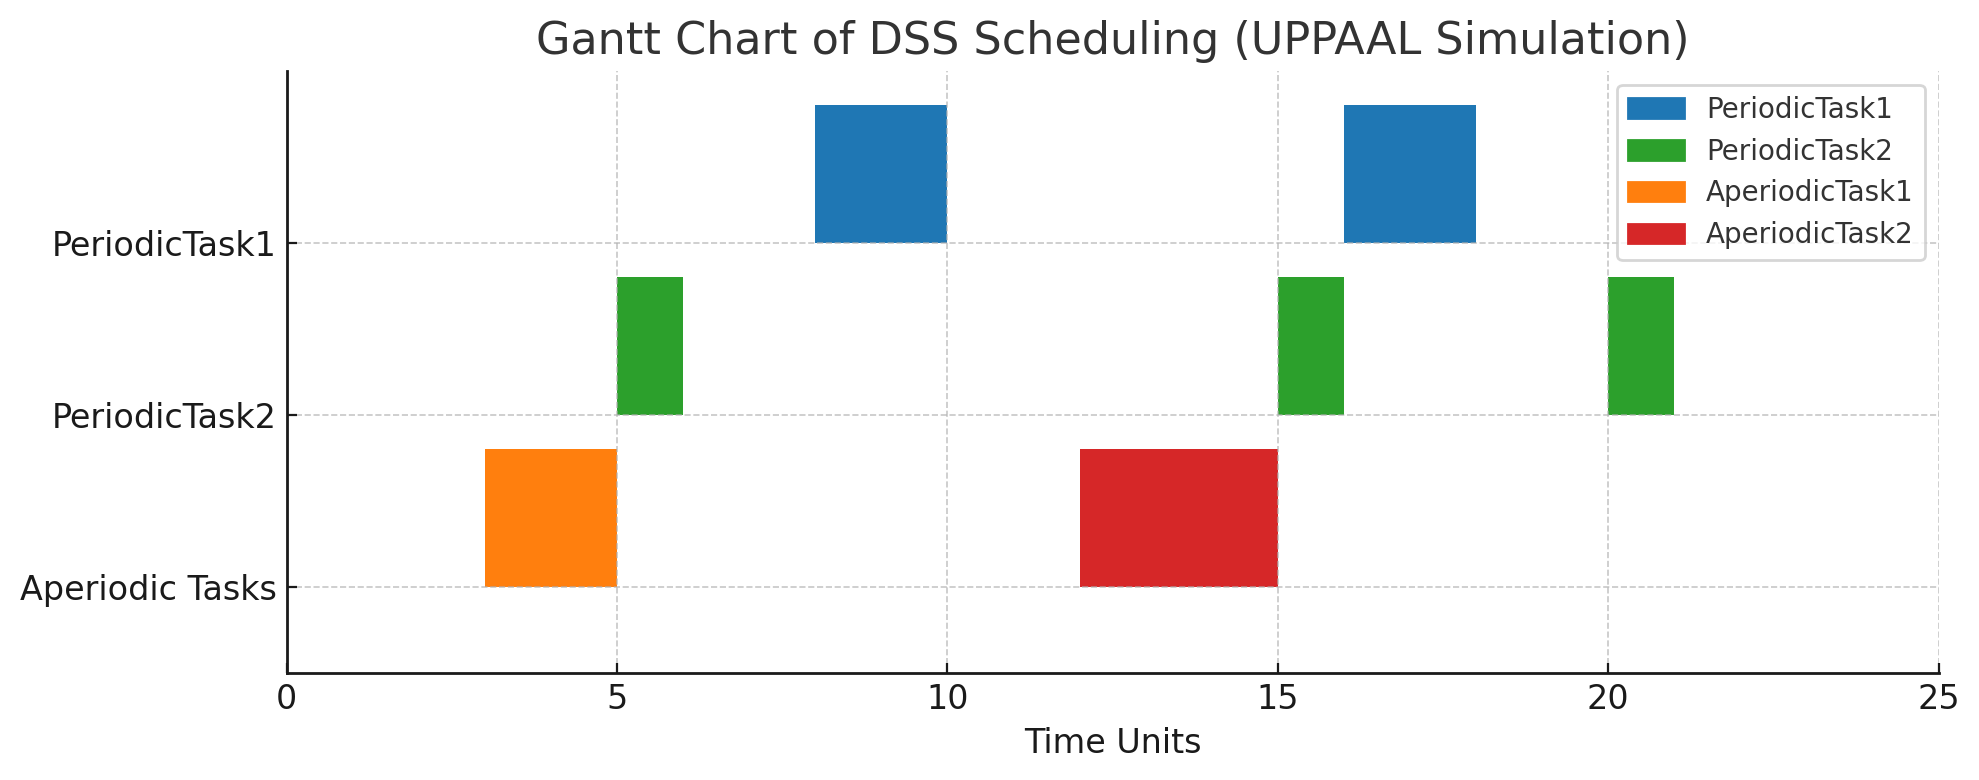
\includegraphics[width=1\linewidth]{06aa5266-f51e-41c8-a4c3-ac8c8555d283.png}
    \caption{Gantt chart}
    \label{fig:enter-label}
\end{figure}
\begin{figure}
    \centering
    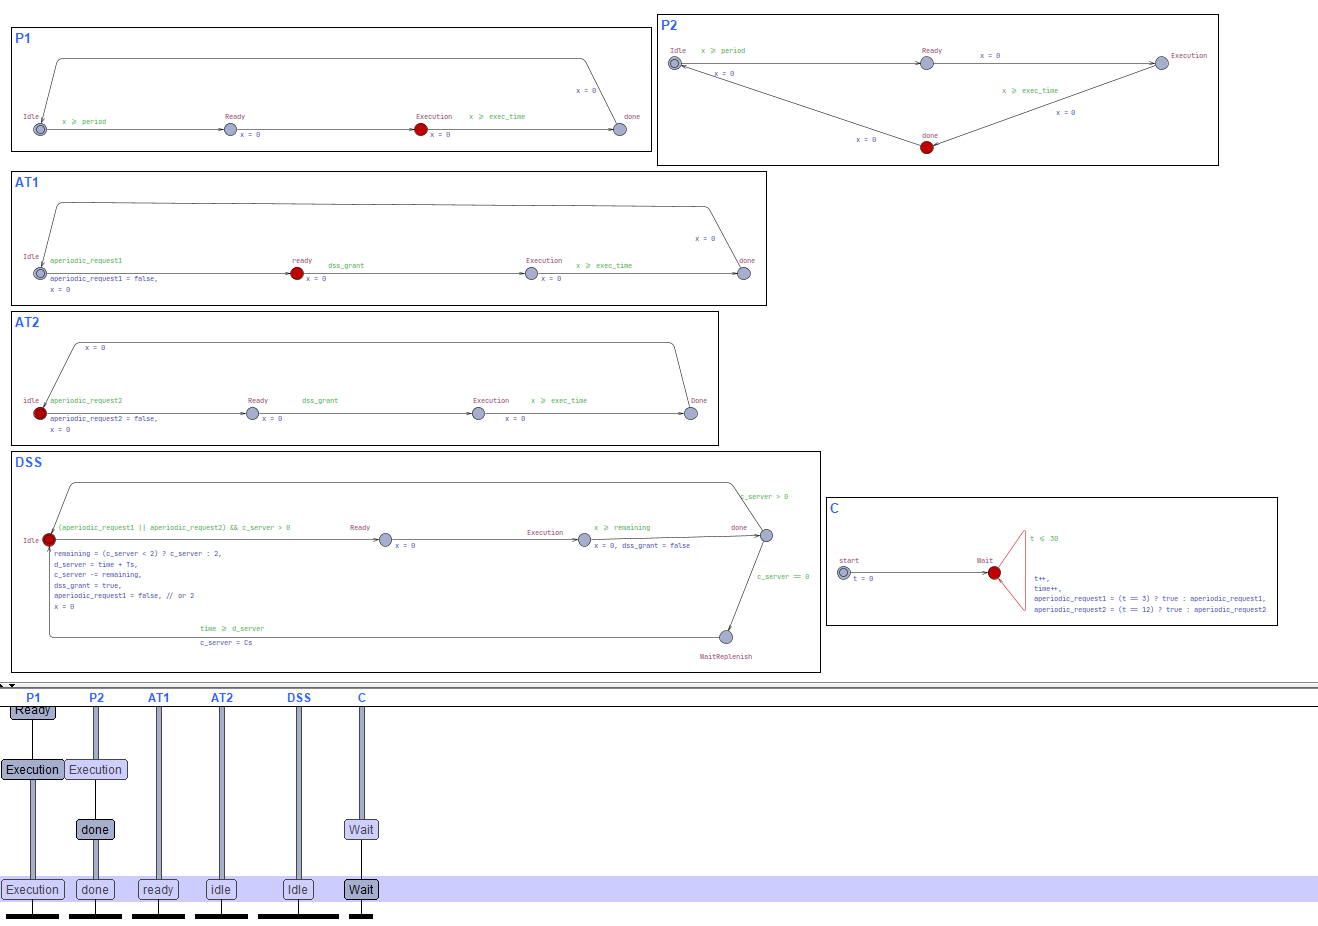
\includegraphics[width=1\linewidth]{Screenshot 2025-05-31 210123.png}
    \caption{Symbolic Simulator}
    \label{fig:enter-label}
\end{figure}
\begin{figure}
    \centering
    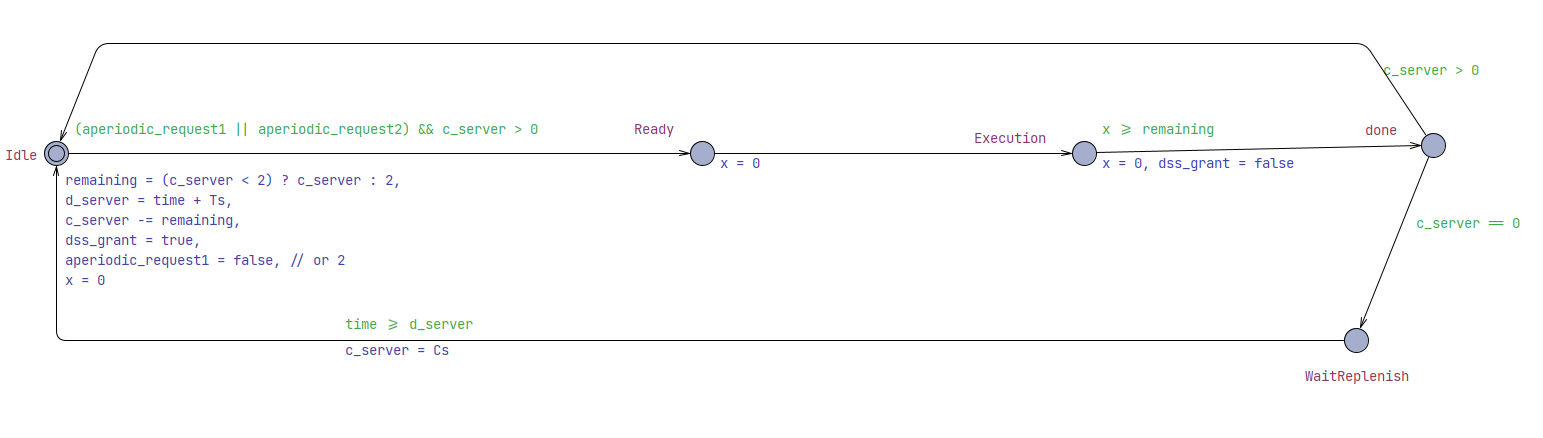
\includegraphics[width=1\linewidth]{DSS Server.png}
    \caption{DSS server}
    \end{figure}
\begin{figure}
    \centering
    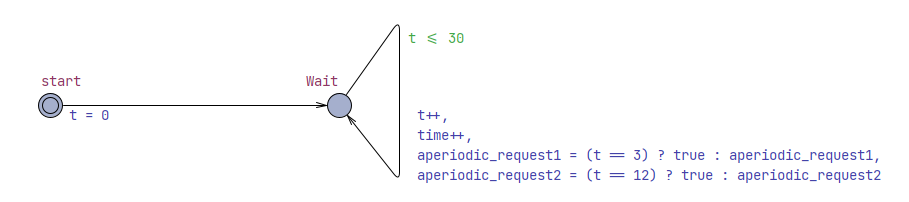
\includegraphics[width=1\linewidth]{Controller.png}
    \caption{Controller}
        \label{fig:enter-label}
\end{figure}
 \begin{figure}
        \centering
        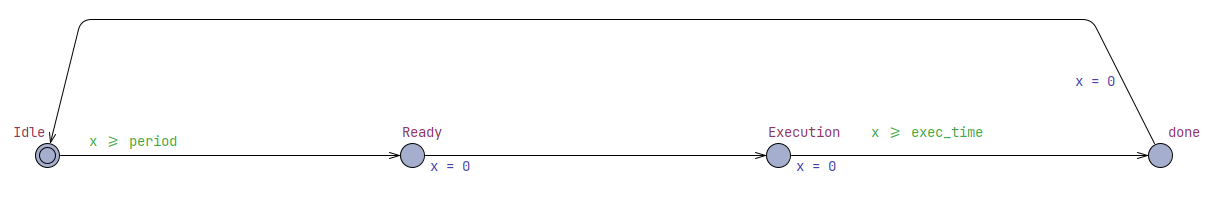
\includegraphics[width=1\linewidth]{PT1.png}
        \caption{Periodic Task 1}
         \label{fig:enter-label}
    \end{figure}
\begin{figure}
            \centering
            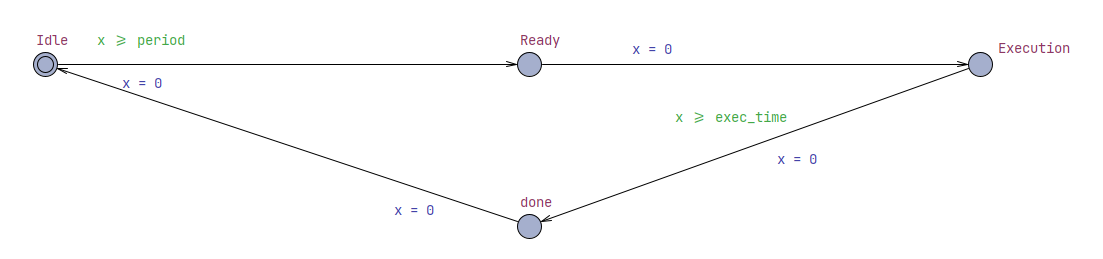
\includegraphics[width=1\linewidth]{PT2.png}
            \caption{Periodic Task 2}
             \label{fig:enter-label}
        \end{figure}
\begin{figure}
                \centering
                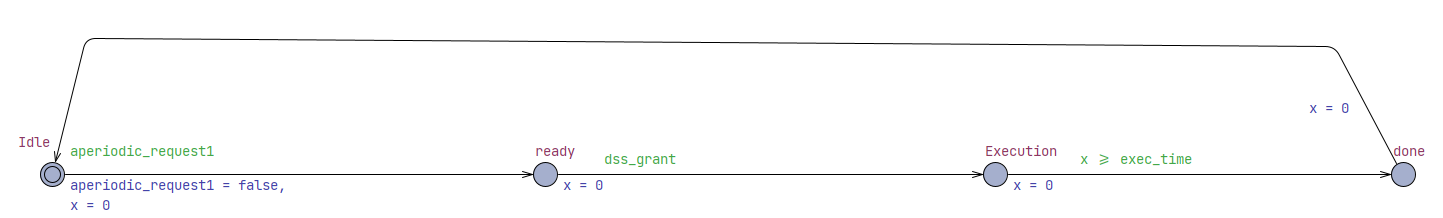
\includegraphics[width=0.75\linewidth]{APT1.png}
                \caption{Aperiodic Task 1}
                \label{fig:enter-label}
            \end{figure}
            \begin{figure}
    \centering
    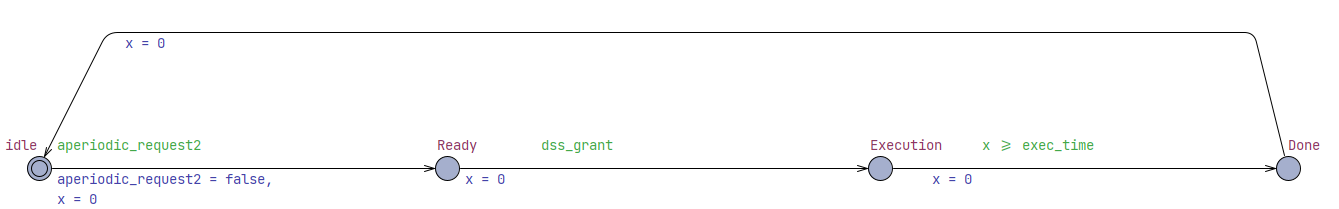
\includegraphics[width=0.75\linewidth]{APT2.png}
    \caption{Aperiodic Task 2}
    \label{fig:enter-label}
\end{figure}
In this seminar, I presented a simulation of the Dynamic Sporadic Server (DSS) model using the UPPAAL tool. The main aim was to show how DSS scheduling can handle aperiodic tasks without interfering with periodic tasks, which is very important in real-time systems. The simulation I made includes two periodic tasks, two aperiodic tasks, a DSS server, and a controller that acts as the environment.

The periodic tasks are designed to run at fixed intervals. \textbf{PeriodicTask1} has a period of 8 time units and executes for 2 time units, while \textbf{PeriodicTask2} has a shorter period of 5 units and executes for 1 time unit. Each periodic task moves through four states: \textit{Idle}, \textit{Ready}, \textit{Execution}, and \textit{Done}. When the period expires, the task moves to \textit{Ready}, then executes for its set time, and then goes to \textit{Done} before resetting.


For the aperiodic part, I included two tasks that are not triggered by time but by events. \textbf{AperiodicTask1} runs for 2 units and is triggered by the controller at time $t = 3$. \textbf{AperiodicTask2} runs for 3 units and is triggered at $t = 12$. However, these tasks can’t just start on their own. They must be allowed by the DSS server through a signal called \texttt{dss\_grant}. This means that even if a request comes in, the task will only run if the DSS says it can.

The \textbf{DSS\_Server} is the key part of the whole model. It manages when and how aperiodic tasks can execute. The server has a capacity ($C_s$) of 3 units, which means it can spend up to 3 time units on aperiodic tasks before it needs to refill. The replenishment period ($T_s$) is 6 units, so every 6 units, it gets its full capacity back. The DSS goes through several states: \textit{Idle} (watching for new requests), \textit{Ready} (when it decides to grant access), \textit{Execution} (running an aperiodic task), \textit{Done} (after the task finishes), and \textit{WaitReplenish} (when it has no capacity and is waiting to refill). It keeps track of how much capacity it has left using the variable \texttt{c\_server} and also remembers when to refill with \texttt{d\_server}.

The \textbf{Controller} in the model is a simple component that simulates the environment. It keeps track of time and triggers the aperiodic task requests at specific points. In my simulation, it sets \texttt{aperiodic\_request1 = true} at $t = 3$ and \texttt{aperiodic\_request2 = true} at $t = 12$. It also increases logical time step by step.

When the simulation runs, both periodic tasks start in \textit{Idle}. At time $t = 3$, the controller triggers the first aperiodic request. Since DSS has full capacity at the start, it grants permission, and \textbf{AperiodicTask1} executes. This reduces the server's capacity by 2 units. Then, periodic tasks keep executing according to their periods \textbf{PeriodicTask2} runs at $t = 5$ and \textbf{PeriodicTask1} at $t = 8$. At $t = 12$, the controller sends the second aperiodic request. Now, depending on how much capacity the DSS has left, it may either run the task or wait until its capacity is replenished.

The simulation clearly shows how DSS works to let aperiodic tasks execute without breaking the schedule of the periodic ones. The DSS carefully tracks how much capacity is used and refills only after the defined period. This method ensures that periodic tasks always get priority and deadlines are not missed, while still giving space to aperiodic tasks when possible. I believe this model demonstrates the concept in a simple but effective way, and helps to understand real-time scheduling more practically.

\section{Comparison with Other Servers}
Table~\ref{tab:servers} compares key features of Polling, Deferrable, Sporadic, and Dynamic Sporadic servers.  Polling servers operate under fixed-priority scheduling and reset their budget at each period regardless of use \cite{sprunt1989aperiodic}.  Deferrable servers also run at high priority but carry unused capacity to the end of the period \cite{buttazzo2011hard}.  The classic Sporadic Server (for Rate-Monotonic scheduling) replenishes only the portion of its budget that was actually consumed \cite{sprunt1989aperiodic}.  


\begin{table}[ht]
\centering
\renewcommand{\arraystretch}{1.1} % Optional: add some vertical spacing
\begin{tabularx}{\columnwidth}{l|X|X|X|X}
\textbf{Feature} & \textbf{Polling} & \textbf{Deferrable} & \textbf{Sporadic} & \textbf{DSS} \\
\hline
Scheduling & Fixed-priority (RM) & Fixed-priority (RM) & Fixed-priority (RM) & Dynamic (EDF) \\\\
Priority & Highest static & Highest static & Static (RM) & Dynamic (deadline $t+T_s$) \\\\
Replenishment & Periodic full & Periodic full & On-demand & On-demand \\\\
Unused Budget & Lost if unused & Carried to period end & Carried to next period & Reused flexibly \\\\
Utilization & Often suboptimal & Improved response & Moderate & Full (up to 100\%) \\\\
\end{tabularx}
\caption{Comparison of Aperiodic Servers}
\label{tab:servers}
\end{table}


DSS stands apart by its EDF-based policy and flexible budget usage.  In practice, DSS provides the responsiveness of a high-priority server without leaving CPU time idle when aperiodic demand is present \cite{buttazzo2011hard, laplante2011real}.

\section{Applications and Use Cases}

Dynamic Sporadic Servers (DSS) are well-suited to systems that must mix hard real-time periodic tasks with unpredictable aperiodic workloads. Typical examples include automotive ECUs, robotic controllers, avionics systems, embedded Linux platforms, multimedia devices, and medical equipment.

For instance, an automotive braking controller may have a periodic speed-monitoring task and a sporadic braking-request task \cite{diva2020ecu}. In such domains, DSS provides a reserved capacity for aperiodic jobs without violating hard deadlines of periodic jobs.

In robotics, a servo loop may run at a fixed rate while sensor or vision processing tasks arrive unpredictably. DSS can absorb these aperiodic jobs using its time-varying deadline mechanism (e.g., “ties are always resolved in favor of the server”) \cite{cpen432}, improving responsiveness without jeopardizing safety-critical loops.

Similarly, avionics flight computers often interleave periodic control tasks (e.g., stabilization) with aperiodic ones (e.g., communication, diagnostics). In multimedia systems, the Linux \texttt{SCHED\_DEADLINE} scheduler uses a variant of DSS (Constant Bandwidth Server) to serve aperiodic workloads (network packets, user interactions) alongside real-time tasks \cite{cpen432}.

In medical systems such as implantable monitors or patient alarms, DSS can isolate life-critical periodic sensing from sporadic events like logging or alarms.

\begin{itemize}
    \item \textbf{Automotive ECUs:} DSS allocates a fixed budget $C_s$ per period $T_s$ to event-driven aperiodic tasks without delaying periodic engine control jobs \cite{diva2020ecu}.
    \item \textbf{Robotics and Control:} DSS enables mixing real-time servo loops with irregular processing (vision/path planning) while meeting EDF feasibility conditions \cite{cpen432}.
    \item \textbf{Avionics:} DSS helps meet deadlines for both periodic sensor/actuator cycles and asynchronous diagnostics.
    \item \textbf{Embedded Linux \& Multimedia:} DSS variants like CBS are used in Linux for EDF-based scheduling of sporadic user interactions or audio/video streams \cite{cpen432}.
    \item \textbf{Medical Systems:} DSS ensures timely response to alarms while maintaining guaranteed periodic monitoring rates.
\end{itemize}

DSS offers strong temporal isolation: aperiodic tasks are treated like a periodic task with utilization $U_s = C_s / T_s$. Spuri and Buttazzo showed that if $U_p + U_s \leq 1$, all EDF deadlines will be met \cite{spuri1994efficient, buttazzo2011hard}.

\section{Limitations and Practical Considerations}

Implementing DSS involves non-trivial complexity. The operating system must manage a dynamic deadline and a replenishable budget. Each aperiodic job arrival or execution requires updating the deadline and tracking consumed capacity \cite{cpen432}. This includes scheduling a replenishment for any consumed portion after $T_s$ time units.

Whenever an aperiodic job executes, it inherits the server’s deadline and may preempt periodic jobs. This makes DSS more complex than simple polling or deferrable servers \cite{cpen432, queensu2023dss}.

In systems using fixed-priority scheduling (e.g., Rate Monotonic), DSS cannot be directly implemented. It relies on EDF for dynamic prioritization. While real-time Linux and some RTOSes support CBS/DSS, integration still requires modifying scheduler internals.

There is also an overhead trade-off: smaller $T_s$ reduces latency but increases context switching. A short $T_s$ means smaller budgets $C_s$, which may lead to queue buildup. Conversely, large $T_s$ values reduce overhead but delay service to aperiodic jobs \cite{queensu2023dss}.

Heavy aperiodic workloads can overwhelm the server. If job arrivals exceed $U_s$, delays increase sharply. Worst-case latency occurs when jobs arrive just after budget exhaustion. System designers must choose $T_s$ and $C_s$ carefully to balance responsiveness with feasibility.

Corner cases also matter. If a server and a periodic job become ready at the same time, tie-breaking policies must prioritize the server \cite{cpen432}. Priority inheritance protocols are needed to avoid deadlocks when tasks share resources. In multicore systems, sharing the server budget across cores further complicates scheduling.

In summary, DSS offers predictability but requires careful implementation and tuning.

\vspace{1em}
\section{Conclusion}

The Dynamic Sporadic Server is a powerful scheduling mechanism that extends EDF by offering guaranteed bandwidth to aperiodic tasks. By dynamically assigning deadlines and replenishing only the used capacity, DSS achieves efficient processor utilization while respecting hard deadlines for periodic tasks \cite{spuri1994efficient, buttazzo2011hard}.

Its strengths include:
\begin{itemize}
    \item Strong temporal isolation and bandwidth reservation.
    \item High responsiveness to aperiodic jobs.
    \item Full utilization up to 100\% under EDF schedulability bounds.
\end{itemize}

DSS is particularly beneficial in mixed-criticality real-time systems such as automotive, avionics, robotics, and embedded Linux environments. Compared to simpler servers, it provides better control and responsiveness, especially under unpredictable workloads.

Looking forward, DSS can be enhanced through variants like the Constant Bandwidth Server (CBS), integration with priority-inheritance protocols, and adaptations for multicore platforms \cite{laplante2011real}. Future research may also explore hybrid EDF-fixed priority schemes and virtualization-aware servers.

In conclusion, DSS remains a relevant and effective solution for real-time systems that require dynamic, predictable aperiodic task management.



\printbibliography


\vspace{12pt}
\color{red}


\end{document}
